\chapter{Introduction}
\label{ch:introduction}

\section{Background and Motivation}
Spaceborne synthetic aperture radar (SAR) systems provide images of the Earth's surface independently of daylight and
cloud cover, and the Copernicus Sentinel-1 constellation delivers C-band acquisitions over most land surfaces every few
days \cite{torres2012,moreira2013}. Image formation in a SAR is based on the measurement of range and Doppler history
rather than on angular projection \cite{curlander1991,cumming2005}. In mountainous terrain this side-looking range
geometry produces characteristic distortions: slopes facing the radar are compressed into few resolution cells
(foreshortening), the top of steep slopes is imaged before their foot (layover), and slopes facing away from the sensor
may not be illuminated at all (radar shadow) \cite{leberl1990,kropatsch1990}. In the Alps these effects affect a large
fraction of every scene and make visual interpretation and quantitative use of the backscatter difficult
\cite{gelautz1998}. Fig.~\ref{fig:intro} illustrates the three effects on a synthetic mountain profile.

\begin{figure}[htbp]
\centering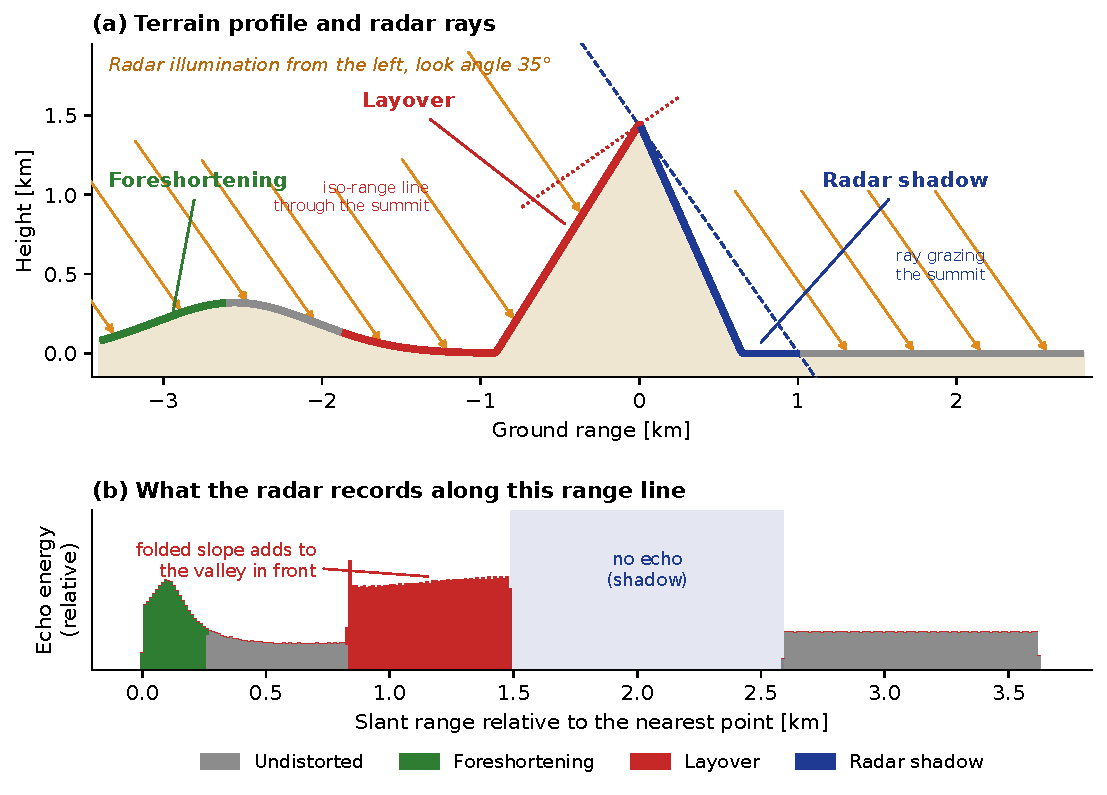
\includegraphics[width=\textwidth]{sar_distortions.pdf}
\caption[Geometric distortions of a side-looking SAR]{Geometric distortions of a side-looking SAR. (a) Terrain profile
illuminated from the left at a look angle of 35$^\circ$: the gentle slope facing the radar is foreshortened, the steep
fore-slope and the valley floor in front of it are in layover, and the back-slope and the terrain behind it lie in
radar shadow. (b) Echo energy recorded along this range line: the foreshortened slope is compressed and bright, the
folded fore-slope is added to the valley floor, and the shadow returns no echo.}
\label{fig:intro}
\end{figure}

Simulating the image that a SAR should record from a digital elevation model (DEM) is the classical way to understand,
predict and correct these effects. DEM-based simulations are used to geocode and terrain-correct SAR data
\cite{schreier1993,meier1993,small2011,low2007}, to generate layover and shadow masks \cite{kropatsch1990}, to estimate
the illuminated area for radiometric normalisation \cite{ulander1996,small2011,frey2013}, and to co-register images
precisely \cite{nitti2011}. Two recent developments make a fresh assessment timely. First, the Copernicus GLO-30 DEM
provides a consistent global elevation model at 1\,arcsec resolution \cite{copdem}. Second, Sentinel-1 Ground Range
Detected (GRD) products are distributed with a complete annotation of orbit state vectors, zero-Doppler timing,
slant-to-ground-range (SRGR) polynomials and radiometric calibration \cite{s1pd}, and are streamed as cloud-optimised
files without registration \cite{planetary}. Together, they allow a simulation to be computed in the exact geometry of a
product and compared with it pixel by pixel.

\section{Problem Statement}
Although DEM-based simulation is an established tool, it is usually embedded in large processing systems whose
internal assumptions are not visible to the user, and it is rarely assessed against real images beyond a visual
comparison. What is less well documented is how far such a DEM-only simulation goes in explaining a real C-band image of
high-relief terrain, which processing choices matter for its geometric and radiometric agreement, and where the
remaining disagreement comes from. A transparent simulator, verified component by component and assessed
quantitatively against real Sentinel-1 data, is required to answer these questions.

\section{Objectives}
The objectives of this work are:
\begin{enumerate}
\item to build a transparent SAR simulator from first principles and verify each of its components quantitatively,
from the impulse response of a point target to a real DEM;
\item to drive the simulator with the annotated geometry of real Sentinel-1 GRD products and assess its geometric
accuracy against the products' own geolocation;
\item to assess the radiometric agreement with the real images for several backscatter laws, for two viewing
geometries and for several processing choices;
\item to identify, with an independent land-cover map, which part of the image a DEM cannot explain.
\end{enumerate}

\section{Scope of the Work}
The study is limited to C-band Sentinel-1 IW GRD products in VV polarisation over one Alpine study site around
Innsbruck, Austria, observed from one ascending and one descending pass. The simulator is an incoherent, single-bounce
image-domain model driven by the Copernicus GLO-30 DEM; double bounce, volume scattering and multi-temporal effects are
outside its scope and are discussed as limitations. All data are open and all software is released with the report.

\section{Organisation of the Report}
The report is organised as follows. Chapter~\ref{ch:literature} reviews SAR image formation, the geometric and
radiometric effects of terrain, and existing SAR simulators. Chapter~\ref{ch:data} describes the study site and the
data. Chapter~\ref{ch:method} presents the raw-signal and image-domain simulators, the range-Doppler geocoding, the
treatment of shadow, layover and radiometry, the comparison strategy and the finalized design.
Chapter~\ref{ch:results} presents and discusses the results, including the limitations of the study.
Chapter~\ref{ch:software} describes the software that implements the work, and Chapter~\ref{ch:conclusions} draws the
conclusions and outlines future work.
